% !TEX encoding = UTF-8
% !TEX TS-program = pdflatex
% !TEX root = ../tesi.tex

%**************************************************************
\chapter{Analisi dei requisiti IW}
\label{cap:analisi-requisiti}
%**************************************************************

\intro{Breve introduzione al capitolo}\\
Questo capitolo ha lo scopo di fornire una definizione dei requisiti individua per la creazione del prodotto Identity Wallet (IW). Le metodologie usate sono tratte dal capitolo quattro di \cite{som:swe}.
Più in particolare la presente capitolo si prefigge di: 
\begin{itemize}
    \item individuare le fonti per la deduzione dei requisiti; 
    \item dedurre i requisiti dalle fonti; 
    \item descrivere i requisiti individuati; 
    \item catalogare i requisiti individuati; 
    \item prioritizzare i requisiti individuati;
\end{itemize}
\section{Specifiche in Linguaggio Naturale}
Il linguaggio naturale ha un’enorme potenza espressiva ma, essendo inerentemente ambiguo, può portare ad incomprensioni. È quindi necessario limitarne l’utilizzo e standardizzarlo, in modo da ridurre al minimo le possibili ambiguità. È comunque fondamentale evitare di utilizzare espressioni e acronimi che possano essere fraintendibili dagli stakeholders, a tal proposito in fondo al documento è presente una lista degli acronimi utilizzato.
\section{Specifiche in Linguaggio Strutturato}
Il linguaggio strutturato mantiene gran parte dell’espressività del linguaggio naturale, fornendo però uno standard schematico che permette l’uniformità della descrizione dei vari requisiti. Sebbene l’utilizzo di un linguaggio strutturato permetta di organizzare i requisiti in modo più ordinato e comprensibile, talvolta la ridotta espressività rende difficile la definizione di requisiti complessi. A tal proposito è possibile integrare la specifica in linguaggio strutturato con una descrizione in linguaggio naturale.
\section{Specifiche in Linguaggio UML Use Case}
Per la definizione dei diagrammi UML dei casi d’uso, viene utilizzato lo standard UML 2.0 \footcite{site:uml}. Nei diagrammi dei casi d’uso vengono mostrati gli attori coinvolti in un’interazione con il sistema in modo schematico, indicando i nomi delle parti coinvolte. Eventuali informazioni aggiuntive possono essere espresse testualmente.


\section{Casi d'uso}

Per lo studio dei casi di utilizzo del prodotto sono stati creati dei diagrammi.
I diagrammi dei casi d'uso (in inglese \emph{Use Case Diagram}) sono diagrammi di tipo \gls{uml} dedicati alla descrizione delle funzioni o servizi offerti da un sistema, così come sono percepiti e utilizzati dagli attori che interagiscono col sistema stesso.

\subsection{Descrizione Attori}
I tipi di attori principali che andranno ad interagire direttamente con il sistema sono essenzialmente tre: 
\begin{itemize}
    \item utente;
    \item utente non registrato;
    \item utente autenticato. 
\end{itemize}   
Tra di essi è presente una relazione di generalizzazione che vede l’attore utente come generalizzazione degli attori utente non registrato e utente registrato. Questo tipo di generalizzazione viene rappresentata graficamente in figura \ref{fig:ger-actors}.
\begin{figure}[!h]
    
    \centering
    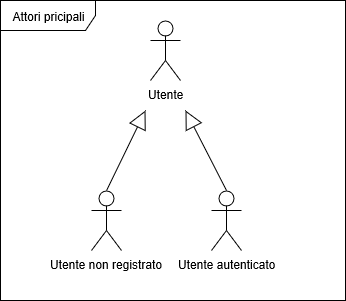
\includegraphics[width=0.5\columnwidth]{usecase/use-case-iw/actors.png} 
    \caption{Gerarchia utenti user case}
    \label{fig:ger-actors} 
\end{figure}
Sono stati individuati i seguenti attori secondari: ITF, MonoKee.
\subsubsection{Attori principali}
\begin{itemize}
    \item \textbf{Utente}: l’attore utente è un fruitore generico del sistema. Potrebbe avere o non avere effettuato l’accesso all’applicazione. Da lui derivano gli attori utente non registrato e utente autenticato.	
    \item \textbf{Utente non registrato}: l’attore utente non registrato è una particolare specializzazione dell’attore utente. Unica sua caratteristica è quella di non essere riconosciuto come utente di MonoKee.
    \item \textbf{Utente autenticato}: l’attore utente autenticato è una particolare specializzazione dell’attore utente. Rappresenta un utente che ha effettuato l’accesso al sistema e che è stato riconosciuto all’interno del sistema MonoKee.
\end{itemize}
      
\subsubsection{Attori secondari}
\begin{itemize}
    \item \textbf{ITF}: è il componente dell’estensione che ha il compito di conservare e convalidare tutte le informazioni provenienti dall’IW.
    \item \textbf{MonoKee}: è il componente centrare dell’attuale servizio MonoKee. Ha il compito di fornire le informazioni di accesso del servizio MonoKee. 
\end{itemize}
    


\subsection{Elenco casi d'uso}


\subsubsection{UC1: Azioni utente generico}
\begin{figure}[!htbp] 
    \centering 
    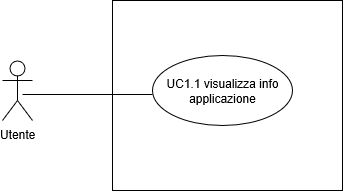
\includegraphics[width=0.7\columnwidth]{usecase/use-case-iw/UC1-azioni-utente.png} 
    \caption{Use Case - UC1: Azioni utente generico}
\end{figure}

\begin{table}[!htbp]
    \caption{Use Case - UC1: Azioni utente generico}
    \label{tab:UC1-Azioni-utente-generico}
    \begin{tabularx}{\textwidth}{|l|X|}
    \hline
    \textbf{Descrizione} & L’utente può visualizzare le informazioni sull’applicazione 
    \\
    \hline
    \textbf{Attore primario} & Utente\\
    \hline
    \textbf{Attore secondario} & Nessuno\\
    \hline
    \textbf{Precondizioni} & L’utente ha avviato l’applicazione\\
    \hline
    \textbf{Postcondizioni} & L’utente ha eseguito le azioni che desiderava compiere in relazione alle sue possibilità\\
    \hline
    \textbf{Scenario principale} & 
        \begin{itemize}
            \item UC1.1 Visualizza info applicazione
        \end{itemize}\\
    \hline
    \textbf{Scenari alternativi} & Nessuno\\
    \hline
    \end{tabularx}
\end{table}



\subsubsection{UC1.1 – Visualizza info applicazione}
\begin{figure}[!htbp] 
    \centering 
    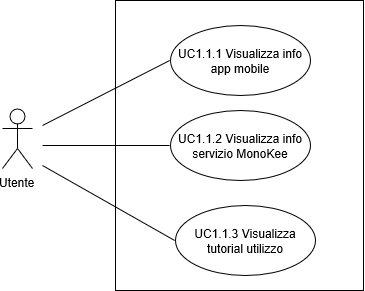
\includegraphics[width=0.7\columnwidth]{usecase/use-case-iw/UC1-1-Visualizza-info-applicazione.png} 
    \caption{Use Case - UC1.1 – Visualizza info applicazione}
\end{figure}

\begin{table}[!htbp]
    \caption{Use Case - UC1.1 – Visualizza info applicazione}
    \label{tab:UC1-Azioni-utente-generico}
    \begin{tabularx}{\textwidth}{|l|X|}
    \hline
    \textbf{Descrizione} & Il sistema deve visualizzare le informazioni relative all’applicazione mobile e al servizio MonoKee
    \\
    \hline
    \textbf{Attore primario} & Utente\\
    \hline
    \textbf{Attore secondario} & Nessuno\\
    \hline
    \textbf{Precondizioni} & L’utente ha avviato l’applicazione\\
    \hline
    \textbf{Postcondizioni} & L’utente ha visualizzato le informazioni che desirava riguardo l’applicazione\\
    \hline
    \textbf{Scenario principale} & 
        \begin{itemize}
            \item UC1.1.1 Visualizza info applicazione
            \item UC1.1.2 Visualizza info servizio MonoKee
            \item UC1.1.3 Visualizza tutorial utilizzo
        \end{itemize}\\
    \hline
    \textbf{Scenari alternativi} & Nessuno\\
    \hline
    \end{tabularx}
\end{table}


\newpage
\section{Tracciamento dei requisiti}

Da un'attenta analisi dei requisiti e degli use case effettuata sul progetto è stata stilata la tabella che traccia i requisiti in rapporto agli use case.\\
Sono stati individuati diversi tipi di requisiti e si è quindi fatto utilizzo di un codice identificativo per distinguerli.\\
Il codice dei requisiti è così strutturato R(F/Q/V)(N/D/O) dove:
\begin{enumerate}
	\item[R =] requisito
    \item[F =] funzionale
    \item[Q =] qualitativo
    \item[V =] di vincolo
    \item[N =] obbligatorio (necessario)
    \item[D =] desiderabile
    \item[Z =] opzionale
\end{enumerate}
Nelle tabelle \ref{tab:requisiti-funzionali}, \ref{tab:requisiti-qualitativi} e \ref{tab:requisiti-vincolo} sono riassunti i requisiti e il loro tracciamento con gli use case delineati in fase di analisi.

\newpage

\begin{table}%
\caption{Tabella del tracciamento dei requisti funzionali}
\label{tab:requisiti-funzionali}
\begin{tabularx}{\textwidth}{lXl}
\hline\hline
\textbf{Requisito} & \textbf{Descrizione} & \textbf{Use Case}\\
\hline
RFN-1     & L'interfaccia permette di configurare il tipo di sonde del test & UC1 \\
\hline
\end{tabularx}
\end{table}%

\begin{table}%
\caption{Tabella del tracciamento dei requisiti qualitativi}
\label{tab:requisiti-qualitativi}
\begin{tabularx}{\textwidth}{lXl}
\hline\hline
\textbf{Requisito} & \textbf{Descrizione} & \textbf{Use Case}\\
\hline
RQD-1    & Le prestazioni del simulatore hardware deve garantire la giusta esecuzione dei test e non la generazione di falsi negativi & - \\
\hline
\end{tabularx}
\end{table}%

\begin{table}%
\caption{Tabella del tracciamento dei requisiti di vincolo}
\label{tab:requisiti-vincolo}
\begin{tabularx}{\textwidth}{lXl}
\hline\hline
\textbf{Requisito} & \textbf{Descrizione} & \textbf{Use Case}\\
\hline
RVO-1    & La libreria per l'esecuzione dei test automatici deve essere riutilizzabile & - \\
\hline
\end{tabularx}
\end{table}%